\documentclass[11pt,a4paper]{article}
\usepackage[margin=25mm]{geometry}
\usepackage{amsmath,amssymb,booktabs}
\usepackage{tikz,pgfplots}
\pgfplotsset{compat=1.18}
\usepackage[hidelinks]{hyperref}
\setlength{\parindent}{0pt}
\setlength{\parskip}{6pt}
\title{Spectral likelihood: oracle-risk scaling experiments}
\author{}
\date{Experiment archive: 27 October 2026}
\begin{document}
\maketitle
\noindent This standalone report provides the numerical section for the v11 ordinary-SBM manuscript. It evaluates the v11 degree-plus-spectrum construction. The older algorithm currently in \texttt{paper/current} on GitHub is a different procedure.
\setcounter{section}{4}
\section{Numerical experiments}\label{sec:experiments}
We examine whether the risk of the complete degree-plus-spectrum algorithm remains within a constant factor of the raw-edge oracle as the graph size increases. The experiment uses the procedure in Section~3.2 of the 27 October v11 manuscript, including its radius-count initialization, degree cap, original-scale reconstruction, zero-diagonal degree correction, symmetric block fit, and simultaneous likelihood updates. It does not use true labels or true probabilities for initialization, fitting, stopping, or model selection.

\subsection{Design and oracle calculation}
For each model and each $n\in\{1000,2000,4000,8000,16000\}$ we generate 20 independent undirected Bernoulli graphs. The community sizes have the proportions below, and vertex labels are randomly permuted before sampling. Write $J_K$ for the $K$-by-$K$ all-ones matrix solely in the following design formulas:
\begin{align*}
\text{Balanced }K=2:\quad &
 (n_1,n_2)/n=(1/2,1/2),\quad P=\frac{4\log n}{n}
 \begin{pmatrix}1&0.35\\0.35&1\end{pmatrix};\\
\text{Unequal }K=3:\quad &
 (n_1,n_2,n_3)/n=(0.40,0.35,0.25),\quad P=\frac{14\sqrt{\log n}}{n}(0.8I_3+0.2J_3);\\
\text{Below-log degree }K=2:\quad &
 (n_1,n_2)/n=(1/2,1/2),\quad P=\frac{1.6\log n}{1.05n}
 \begin{pmatrix}1&0.05\\0.05&1\end{pmatrix}.
\end{align*}
The last model has expected degree
$0.8\log n-1.6\log n/(1.05n)<\log n$ at every tested size.
The three-community model has expected degrees of order $\sqrt{\log n}$.
All three use positive block probabilities and a fixed nondegenerate normalized block matrix.

We fix $b_0=4$ and $c_0=0.02$ throughout and perform ten completed fits and simultaneous label updates. No initialization restarts or raw-edge refinement steps are added. For each graph we compute the misclassification proportion after one global permutation of the estimated labels.

The denominator is the average multiclass oracle error defined in Section~2 of v11. In particular, it is neither a Chernoff-exponent approximation nor the error of a fitted raw-edge procedure. Conditional on a tested vertex's true class, its incident block counts are independent binomials with the self-excluded community sizes. We sum their product probabilities over the count vectors misclassified by the same full edge-and-nonedge likelihood rule and fixed tie ordering. The binomial sums are evaluated numerically; the discarded tail probability is bounded by a decreasing-ratio geometric bound, below $6\times10^{-57}$ in all 15 conditions. This bound concerns truncation, not floating-point rounding.

Each reported numerator averages 20 whole-graph misclassification proportions. The 95\% intervals use the empirical standard deviation across these graphs and the $t_{19}$ critical value; we divide their endpoints by the deterministic oracle risk. Vertices within a graph are not treated as independent replicates.

\subsection{Risk relative to the oracle}
Table~\ref{tab:oracle-scaling} and Figure~\ref{fig:oracle-scaling} give all conditions. There are 300 graphs and 1.86 million classified vertices in total.
\begin{table}[!htbp]
\centering
\small
\caption{Mean algorithmic risk and numerically evaluated Bernoulli oracle risk, both in percent. The last column is the graphwise 95\% interval for their ratio. Every row contains 20 independent graphs.}\label{tab:oracle-scaling}
\begin{tabular}{@{}lrrrrr@{}}
\toprule
Model & $n$ & Algorithm (\%) & Oracle (\%) & Ratio & 95\% interval\\
\midrule
\addlinespace
Balanced $K=2$ & 1,000 & 3.215 & 1.110 & 2.90 & $[2.66,3.14]$ \\
 & 2,000 & 2.143 & 0.867 & 2.47 & $[2.31,2.63]$ \\
 & 4,000 & 1.799 & 0.675 & 2.67 & $[2.52,2.81]$ \\
 & 8,000 & 1.328 & 0.524 & 2.54 & $[2.40,2.68]$ \\
 & 16,000 & 1.044 & 0.406 & 2.57 & $[2.50,2.65]$ \\
\addlinespace
Unequal $K=3$ & 1,000 & 1.115 & 0.553 & 2.01 & $[1.69,2.33]$ \\
 & 2,000 & 1.123 & 0.474 & 2.37 & $[2.15,2.59]$ \\
 & 4,000 & 0.905 & 0.434 & 2.08 & $[1.93,2.24]$ \\
 & 8,000 & 0.753 & 0.379 & 1.98 & $[1.87,2.10]$ \\
 & 16,000 & 0.643 & 0.312 & 2.06 & $[1.99,2.14]$ \\
\addlinespace
Below-log $K=2$ & 1,000 & 1.345 & 0.216 & 6.22 & $[5.39,7.04]$ \\
 & 2,000 & 0.945 & 0.156 & 6.06 & $[5.41,6.71]$ \\
 & 4,000 & 0.720 & 0.112 & 6.43 & $[5.89,6.97]$ \\
 & 8,000 & 0.475 & 0.080 & 5.92 & $[5.37,6.46]$ \\
 & 16,000 & 0.344 & 0.057 & 5.98 & $[5.69,6.27]$ \\
\bottomrule
\end{tabular}
\end{table}
\begin{figure}[t]
\centering
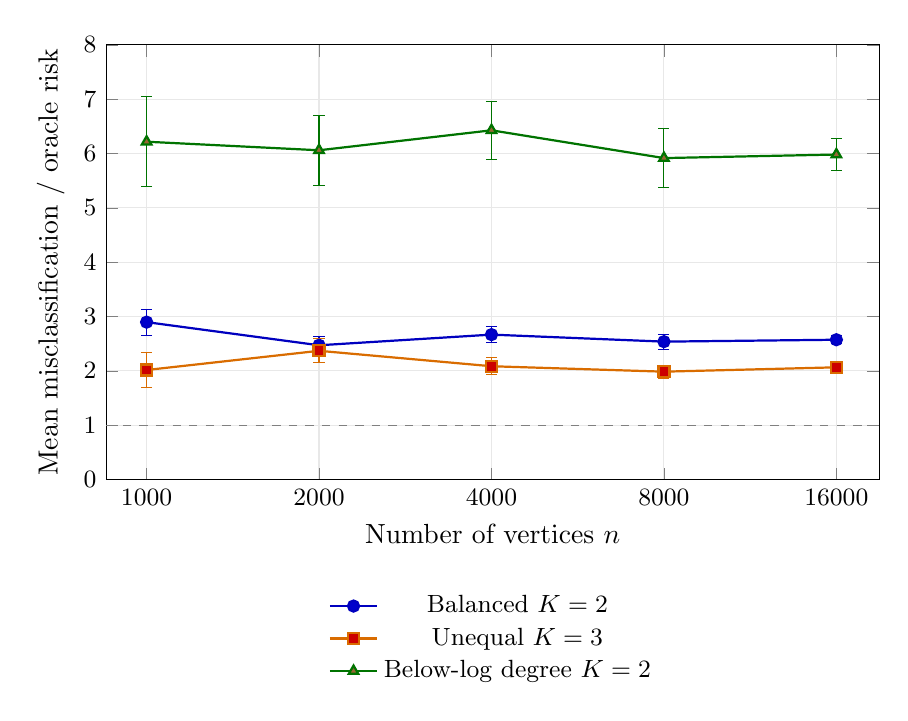
\begin{tikzpicture}
\begin{semilogxaxis}[
 width=0.94\textwidth,height=7.1cm,
 log basis x=2,
 xmin=850,xmax=19000,ymin=0,ymax=8,
 xtick={1000,2000,4000,8000,16000},
 xticklabels={1000,2000,4000,8000,16000},
 xlabel={Number of vertices $n$},
 ylabel={Mean misclassification / oracle risk},
 ytick={0,1,2,3,4,5,6,7,8},
 grid=major,grid style={gray!18},
 legend style={at={(0.5,-0.24)},anchor=north,draw=none,font=\small},
 legend columns=1,
 tick label style={font=\small},
]
\addplot[gray,dashed,forget plot,domain=850:19000] {1};
\addplot+[blue!75!black,mark=*,thick,error bars/.cd,y dir=both,y explicit] coordinates {
(1000,2.895910501) +- (0,0.2393631833)
(2000,2.469985512) +- (0,0.1619304744)
(4000,2.666094515) +- (0,0.1482758664)
(8000,2.536875006) +- (0,0.1391395183)
(16000,2.571807680) +- (0,0.07512064107)
};
\addlegendentry{Balanced $K=2$}

\addplot+[orange!85!black,mark=square*,thick,error bars/.cd,y dir=both,y explicit] coordinates {
(1000,2.014531142) +- (0,0.3202614256)
(2000,2.368148439) +- (0,0.2216389244)
(4000,2.083940025) +- (0,0.1538064472)
(8000,1.984009845) +- (0,0.1174256180)
(16000,2.064020141) +- (0,0.07116271720)
};
\addlegendentry{Unequal $K=3$}

\addplot+[green!45!black,mark=triangle*,thick,error bars/.cd,y dir=both,y explicit] coordinates {
(1000,6.217708555) +- (0,0.8260211796)
(2000,6.060227929) +- (0,0.6457397083)
(4000,6.427724200) +- (0,0.5386154890)
(8000,5.916451084) +- (0,0.5468295707)
(16000,5.981884629) +- (0,0.2898331924)
};
\addlegendentry{Below-log degree $K=2$}

\end{semilogxaxis}
\end{tikzpicture}
\caption{Risk ratios across graph sizes. Error bars are 95\% intervals based on independent graphs. The dashed reference line is one.}\label{fig:oracle-scaling}
\end{figure}

For the balanced two-community model, the ratio ranges from 2.47 to 2.90 and is 2.57 at the largest size. For unequal three-community sizes it ranges from 1.98 to 2.37 and is 2.06 at the largest size. The below-log-degree model has a larger loss, with ratios from 5.92 to 6.43 and a largest-size ratio of 5.98. Thus the measured ratios remain of constant order over the tested range, including the below-log-degree example. These finite simulations support the constant-factor objective; they do not establish an asymptotic bound or its uniformity over all admissible block matrices.

Likelihood updates reduce the three-community error from 1.845\% to 1.115\% at $n=1000$, and from 1.086\% to 0.643\% at $n=16000$. In the symmetric two-community models the radius initializer is already close to the final output, and the refits do not systematically improve its error. We retain these outcomes rather than selecting an update count using true labels.

\subsection{Implementation checks and limitations}
All 300 prescribed runs completed, with no fallback partitions, numerical-solver failures, or discarded main runs. The largest relative eigenpair residual was below $10^{-7}$ and the largest degree-preservation residual was $4.7\times10^{-13}$. Independent small-matrix checks compare factorized counts, symmetric parameter fits, and classification scores against explicit entrywise calculations. The binomial oracle is also checked against exhaustive enumeration of all 128 possible incident rows at $n=8$. An active-cap star graph with isolated vertices verifies original-scale reconstruction and the retention of a negative informative eigenvalue; exact spatial-tree radius counts are checked against brute force.

The degree cap was inactive on the 300 main graphs, so these simulations alone do not assess its benefit for extreme-degree realizations. The three model families were fixed after pilot design checks and before running the main seeds. Two earlier three-community pilot designs, including one numerical nonconvergence and one oracle risk too small for the intended sample budget, are documented in the archive. They are not counted among the 300 main graphs. Code, seeds, oracle calculations, per-graph error traces, numerical diagnostics, and all summary rows are supplied with this section.

\end{document}
